\documentclass{scrartcl}
\usepackage{graphicx}
\graphicspath{ {../images/} }
\usepackage{lipsum}
    \usepackage{subfig} % Um mehrere Bilder nebeneinander

\renewcommand\floatpagefraction{0.1}

\makeatletter
\renewcommand*\fps@figure{p}
\@fpsep\textheight
\makeatother

\begin{document}

\lipsum[10-40]

\begin{figure}
        \centering{}
% \captionsetup{justification=centering}
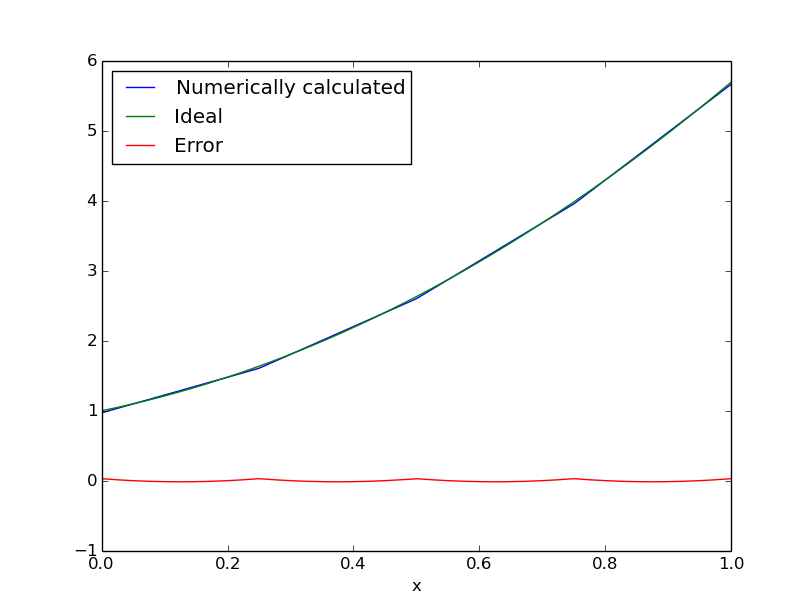
\includegraphics[width=2in]{allmw4.png}
\caption{\label{fig:allmw4}LLMW wavelet: Solution and Error in solution of Equation \ref{eq:analytical} with $n=4$}
\end{figure}

\begin{figure}
        \centering{}
% \captionsetup{justification=centering}
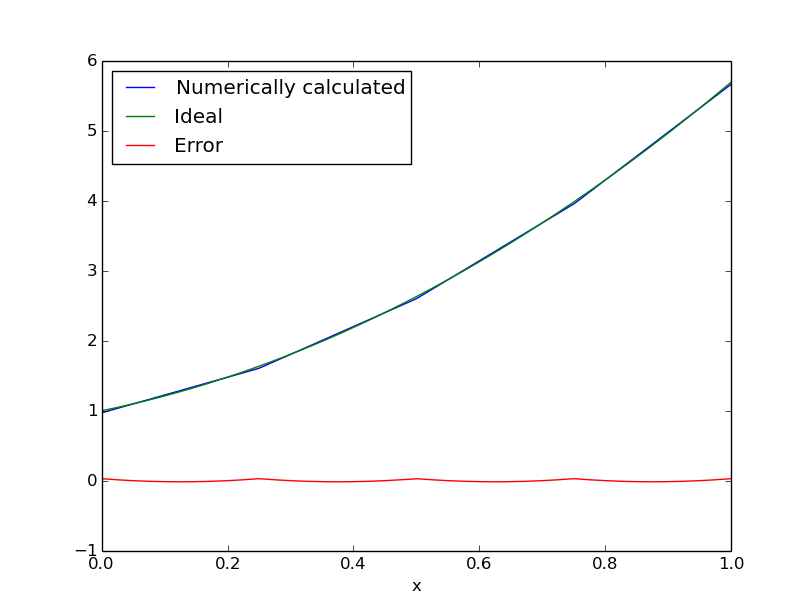
\includegraphics[width=2in]{allmw4.png}
\caption{\label{fig:allmw4}LLMW wavelet: Solution and Error in solution of Equation \ref{eq:analytical} with $n=4$}
\end{figure}

\begin{figure}
        \centering{}
% \captionsetup{justification=centering}
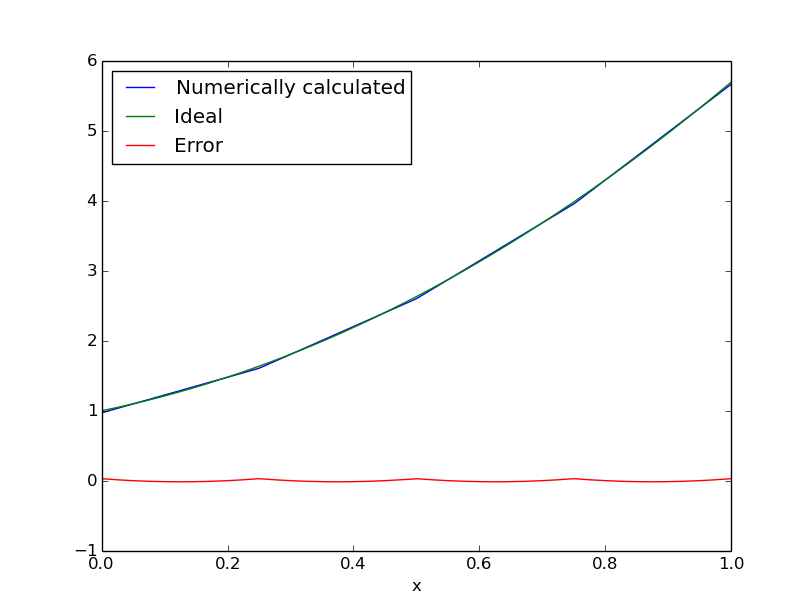
\includegraphics[width=2in]{allmw4.png}
\caption{\label{fig:allmw4}LLMW wavelet: Solution and Error in solution of Equation \ref{eq:analytical} with $n=4$}
\end{figure}

\begin{figure}
        \centering{}
% \captionsetup{justification=centering}
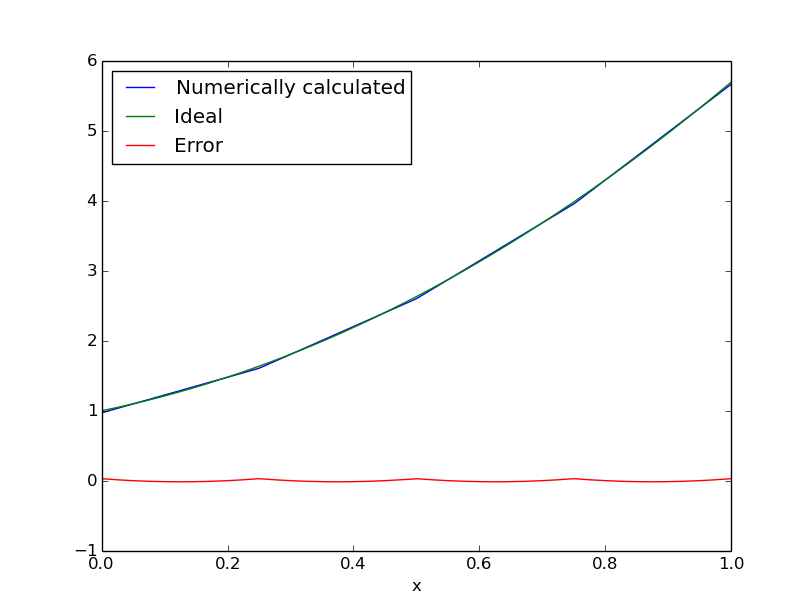
\includegraphics[width=2in]{allmw4.png}
\caption{\label{fig:allmw4}LLMW wavelet: Solution and Error in solution of Equation \ref{eq:analytical} with $n=4$}
\end{figure}

\begin{figure}
        \centering{}
% \captionsetup{justification=centering}
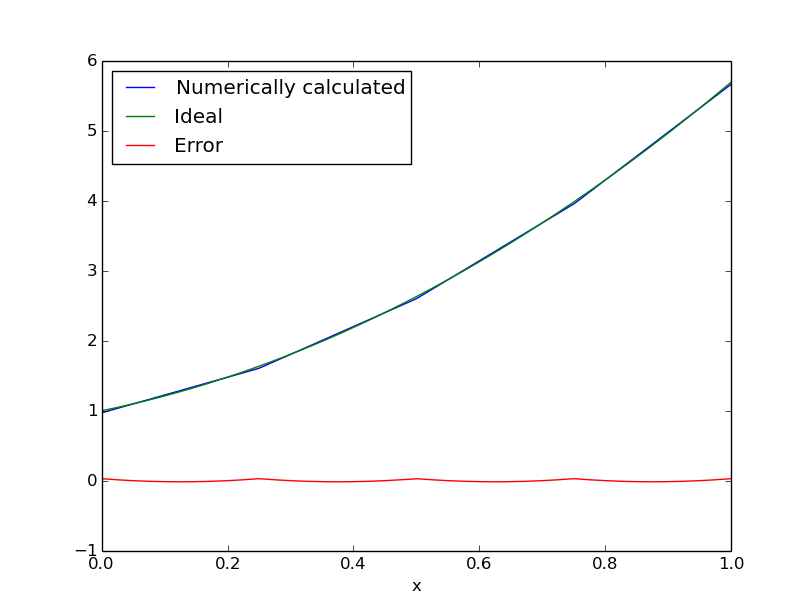
\includegraphics[width=2in]{allmw4.png}
\caption{\label{fig:allmw4}LLMW wavelet: Solution and Error in solution of Equation \ref{eq:analytical} with $n=4$}
\end{figure}
\begin{figure*}
\centering
\subfloat[Mother Wavelet Function: $\phi(x)$]{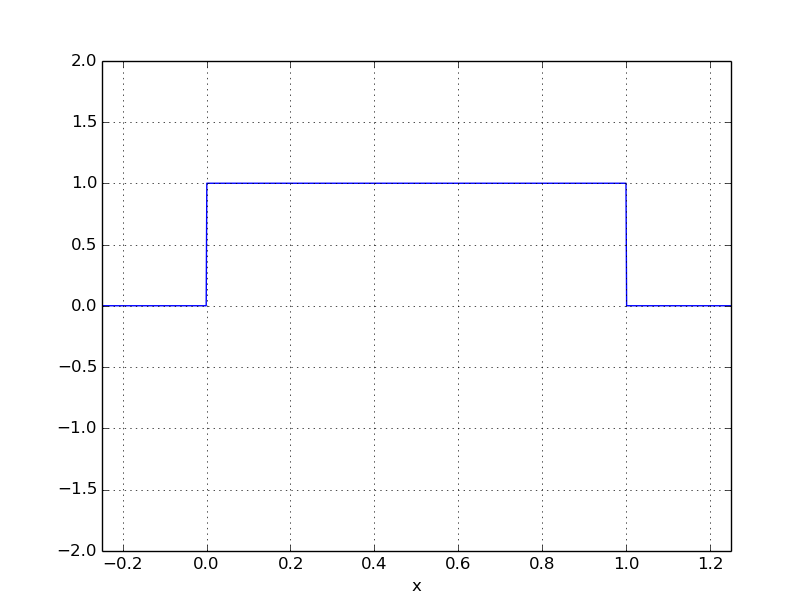
\includegraphics[width=5in]{haarphi.png}
\label{fig:haarphi}
}
\newline
\subfloat[Scaling Function: $\psi(x)$]{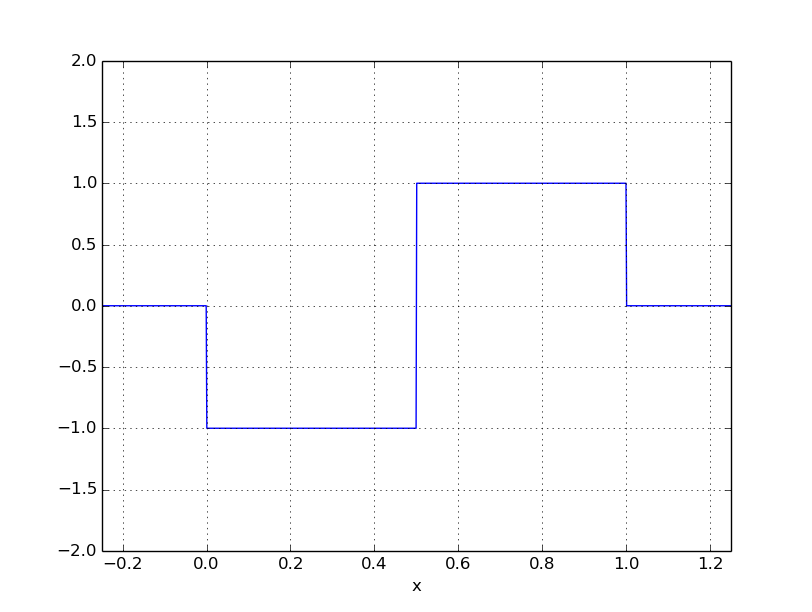
\includegraphics[width=5in]{haarpsi.png}
\label{fig:haarpsi}
}\\
\caption{Haar Wavelet}
\label{fig:haarphipsi}
\end{figure*}

\begin{figure}
        \centering{}
% \captionsetup{justification=centering}
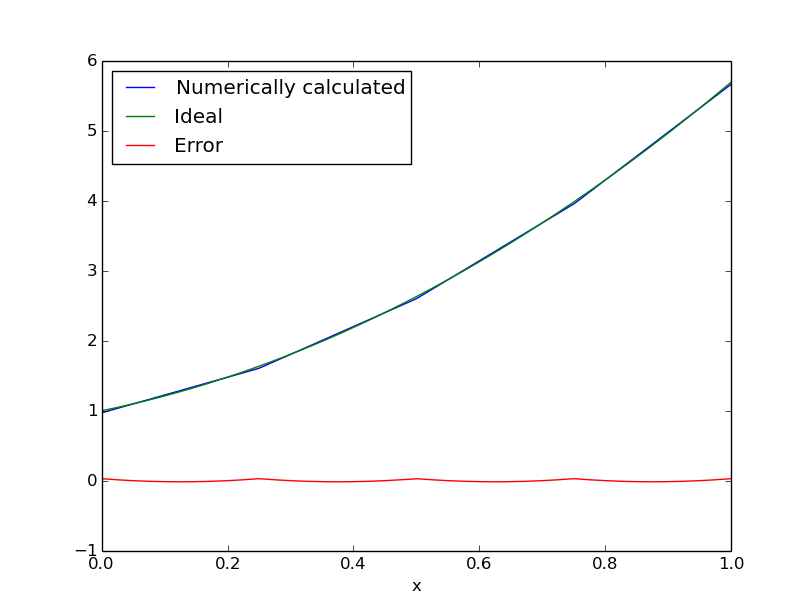
\includegraphics[width=2in]{allmw4.png}
\caption{\label{fig:aqlmw4}LLMW wavelet: Solution and Error in solution of Equation \ref{eq:analytical} with $n=4$}
\end{figure}

\begin{figure}
        \centering{}
% \captionsetup{justification=centering}
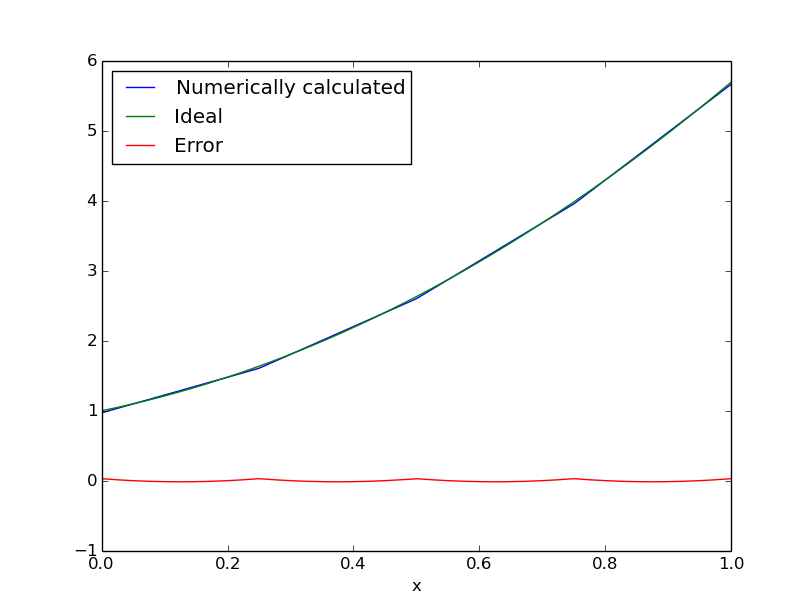
\includegraphics[width=2in]{allmw4.png}
\caption{\label{fig:allmw4}LLMW wavelet: Solution and Error in solution of Equation \ref{eq:analytical} with $n=4$}
\end{figure}

\begin{figure}
        \centering{}
% \captionsetup{justification=centering}
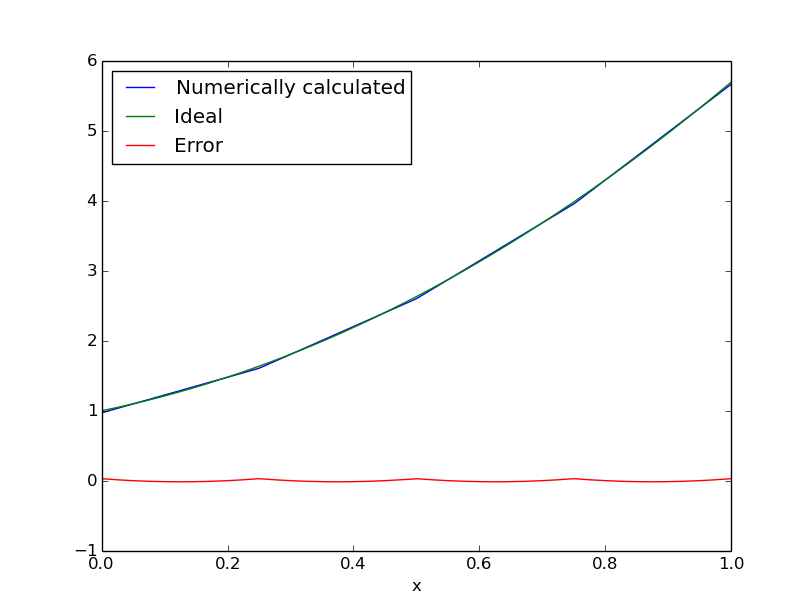
\includegraphics[width=2in]{allmw4.png}
\caption{\label{fig:allmw4}LLMW wavelet: Solution and Error in solution of Equation \ref{eq:analytical} with $n=4$}
\end{figure}

\lipsum[50-80]

\begin{figure}
        \lipsum[2]
\end{figure}

\lipsum[90-120]

\end{document}